%% LaTeX2e class for student theses
%% sections/content.tex
%% 
%% Karlsruhe Institute of Technology
%% Institute for Program Structures and Data Organization
%% Chair for Software Design and Quality (SDQ)
%%
%% Dr.-Ing. Erik Burger
%% burger@kit.edu
%%
%% Version 1.3.6, 2022-09-28

\chapter{Einleitung}
\label{ch:Introduction}


\todo{Ist hier irgendwas spezifisch zu Unit Tests? Die sind nicht mehr Inhalt dieser Arbeit.}

% testen ist wichtig

Das Testen von Software ist ein wichtiger Bestandteil der Softwareentwicklung, der sicherstellt, dass die Software wie erwartet funktioniert und die festgelegten Anforderungen erfüllt.
Es gibt verschiedene Arten von Softwaretests, darunter Unit-Tests, Systemtests und Akzeptanztests \cite{Sommerville10}.
Im Folgenden wird der Fokus auf funktionale Systemtests von Webanwendungen gelegt, die die gesamte Anwendung testen und dabei als Blackbox betrachten \cite{Beizer1990}.
Diese werden in Kapitel \ref{sec:Foundations:GUIBasedSystemTests} näher beschrieben.

% testen speziell von GUIs ist wichtig

Zumindest einzelne Komponenten einer Webanwendung werden gewöhnlich in dem Webbrowser des Benutzers ausgeführt, in dem die Anwendung auch dargestellt wird.
Dadurch ergeben sich besondere Herausforderungen für das Testen von Webanwendungen.
Einerseits verschärfen die Ausführung von Anwendungscode und Darstellung im Browser das Problem der Flakiness, bei der Tests kein konsistentes Ergebnis liefern, auch wenn die Anwendung nicht geändert wurde.
Gleichzeitig bedeuten Änderungen an der graphischen Benutzeroberfläche (Englisch: graphical user interface, GUI) oft, dass auch die Tests geändert werden müssen \cite{ChallengesSelenium}.
Lösungsansätze für diese Probleme sind Gegenstand aktiver Forschung, eine Auswahl wird in Kapitel \ref{ch:RelatedWork} vorgestellt.

% es wäre schön, wenn Tests ohne hartkodierte Fehlerbedingungen Fehler erkennen könnten

Diese Arbeit schließt an die Arbeit von \Citeauthor{GPT3Testing} an.
Ihr Ansatz ermöglicht das automatische Testen über GUIs, was sie an einer einfachen Webanwendung evaluieren.
Sie verwenden ein großes Sprachmodell (Englisch: large language model, LLM), um Benutzerinteraktionen zu generieren, mit denen die Anwendung getestet wird.
Dabei handelt es sich um eine Anwendung aus dem Bereich des maschinellen Lernens, die in der Lage ist, kontextuell angemessene Antworten auf eine Vielzahl von Aufgaben zu generieren \cite{FewShotLearners}.
Das LLM bekommt eine strukturierte Repräsentation der graphischen Benutzeroberfläche, vorherige Benutzerinteraktionen und eine natürlichsprachliche Testbeschreibung als Eingabe.
Es wird aufgefordert, eine Benutzerinteraktion zu generieren, die anschließend automatisch in der Anwendung ausgeführt wird \cite{GPT3Testing}.

In den Kapiteln \ref{ch:ExperimentalSetup} und \ref{ch:Results} liefert diese Arbeit zwei Beiträge:
Erstens wird der Ansatz an einer komplexeren Webanwendung mit verschiedenen Möglichkeiten zur Interaktion getestet.
Zweitens wird untersucht, ob das LLM gleichzeitig als Testorakel verwendet werden kann, das heißt, ob das LLM auch in der Lage ist, Fehlerzustände zu erkennen.

\todo{Absatz über \ref{ch:Conclusion}}

Zuletzt befindet sich in Anlage \ref{ch:PracticalNotes} eine Sammlung von Erkenntnissen, die sich im Verlauf dieser Arbeit gezeigt haben und die für den praktischen Einsatz hilfreich sein könnten.


% LLMs sind vielversprechend \cite{GPT3Testing}, 

\chapter{Grundlagen}
\label{ch:Foundations}

\section{Systemtests auf Grundlage von graphischen Benutzeroberflächen}
\label{sec:Foundations:GUIBasedSystemTests}
Softwaretests sind ein wesentlicher Bestandteil der Softwareentwicklung.
\todo{Er oder sie} umfasst die Bewertung einer Softwareanwendung oder eines Systems, um etwaige Mängel oder Fehler zu erkennen, die die Funktionalität, Zuverlässigkeit oder Leistung beeinträchtigen könnten.
Das Ziel von Softwaretests ist es, sicherzustellen, dass die Software wie erwartet funktioniert und die festgelegten Anforderungen erfüllt.
Es gibt verschiedene Arten von Softwaretests, darunter Unit-Tests, Integrations-Tests, Systemtests und Akzeptanztests.
Das Testen eines GUI-basierten Systems, bei dem nur auf die GUI zugegriffen wird, nennen wir einen GUI-basierten Systemtest oder GUI-Test.
Es wird oft von Software-Testern oder Qualitätssicherungsexperten durchgeführt, die eine Kombination aus manuellen und automatisierten Testmethoden benutzen, um Fehler zu erkennen und sicherzustellen, dass die Software die gewünschten Qualitätsstandards erfüllt.
Manuelle Tests sind ein gängiger Ansatz für GUI-basierte Systemtests, bei denen Tester Testfälle manuell ausführen, Benutzeraktionen simulieren und Beobachtungen und Feedback aufzeichnen.
Es können auch automatisierte Testtools wie Selenium und Appium verwendet werden, um GUI-Tests zu automatisieren, wodurch die Effizienz und Genauigkeit des Testprozesses erhöht werden kann.

GUI-Tests können grob in exploratives Testen und Testen auf der Grundlage von Designer-Testfällen unterteilt werden.
Beim explorativen Testen besteht das Ziel in der Regel darin, Pfade in der zu testenden Anwendung (Englisch: application under test, AUT) zu finden, die zu Abstürzen führen.
Eine grundlegende Technik für exploratives Testen, die leicht automatisiert werden kann, ist das Monkey-Testing, bei dem zufällige Benutzeraktionen simuliert werden.
Im Gegensatz dazu sind Tests, die von Designern spezifiziert werden, oft sehr viel kostspieliger.
Um diese zu automatisieren, müssen die Programmierer aus der Spezifikation Testskripte ableiten, die parallel zu Änderungen an der graphischen Benutzeroberfläche gewartet werden müssen.
Dies ist ein Problem, da die graphische Benutzeroberfläche oft der sich am häufigsten ändernde Teil eines Systems ist.

\section{Metriken für die Testabdeckung}
\label{sec:Foundations:TestCoverageMetrics}

Die Testabdeckung ist eine Metrik, die die Menge des Quellcodes oder der Anwendungszustände misst, die durch Tests abgedeckt wird \cite{Sommerville10}.
Ein Ziel der Testabdeckungsmetriken ist es, die Qualität der Tests zu bewerten  und sicherzustellen, dass es keine ungetesteten Teile des Codes gibt.
Es folgt eine kurze Übersicht über die gängigsten Metriken für die Testabdeckung.

\begin{itemize}
    \item 
    Funktionsabdeckung: Die Funktionsabdeckung misst den Anteil der Funktionen die durch Tests ausgeführt werden.
    Sie zeigt an, ob zumindest alle Funktionen des Quellcodes einmal durchlaufen werden.
    Vorteil der Funktionsabdeckung ist, dass sie einfach zu verstehen und zu implementieren ist und hilft, ungetestete Funktionen zu identifizieren.
    Sie ist nützlich für funktionale Programmiersprachen und Projekte mit sauberer Modularisierung in kleine Funktionen ohne viele Kontrollstrukturen und Seiteneffekte.
    Nachteilig ist, dass keine Aussage über die Abdeckung innerhalb der Funktionen getroffen wird.
    \item
    Zeilenabdeckung: Die Zeilenabdeckung misst, den Anteil der Zeilen des Quellcodes durch Tests abgedeckt werden.
    Sie ist ein Indikator dafür, welche Zeilen des Quellcodes während der Ausführung der Tests zumindest einmal durchlaufen werden.
    Vorteil der Zeilenabdeckung ist, dass sie einfach zu verstehen und zu implementieren ist und eine grundlegende Aussage über die Testabdeckung liefert.
    Nachteilig ist, dass sie Kontrollstrukturen wie Schleifen und Verzweigungen innerhalb von Zeilen nicht berücksichtigt und somit Code der nicht getestet wird, als getestet markieren kann.
    \item
    % statements
    Anweisungsabdeckung: Die Anweisungsabdeckung misst den Anteil einzelner Anweisungen des Quellcodes, die durch Tests abgedeckt werden.
    Dafür wird jede Anweisung des Quellcodes gezählt und die Anzahl der Anweisungen, die durch Tests abgedeckt werden, ins Verhältnis gesetzt.
    Die Anweisungsabdeckung ist eine feinere Metrik als die Zeilenabdeckung, da sie auch die Abdeckung von Anweisungen innerhalb von Kontrollstrukturen berücksichtigt.
    Eine verhältnismäßig hohe Anweisungsabdeckung kann jedoch auch erreicht werden, wenn nur die Fälle mit den meitsten Anweisungen getestet werden.
    % branch
    \item 
    Verzweigungsabdeckung: Die Verzweigungsabdeckung misst den Anteil der Verzweigungen des Quellcodes, die durch Tests abgedeckt werden.
    Es misst ob jeweils alle Zweige einer Kontrollflussstruktur (z.B. \textit{if} oder \textit{switch-case} Strukturen) durchlaufen werden.
    Die Verzweigungsabdeckung ist genauso fein wie die Anweisungsabdeckung, aber gibt einen besseren Einblick in die Ausführlichkeit der Tests in Bezug auf Fallunterscheidungen.
    Sie hilft dabei Verzweigungen zu identifizieren, die nicht getestet werden.
    % path
    \item
    Pfadabdeckung: Die Pfadabdeckung misst den Anteil der Pfade durch den Quellcode, die durch Tests abgedeckt werden zu denen die theoretisch möglich sind.
    Sie ist die feinste mögliche Metrik für die Testabdeckung, da sie alle möglichen Pfade durch den Quellcode berücksichtigt.
    Sie ist jedoch auch die aufwändigste Metrik, da sie alle möglichen Pfade durch den Quellcode berücksichtigt.
    Je nach Komplexität des Quellcodes kann die Pfadabdeckung sehr aufwändig zu berechnen sein und es kann auch unendlich viele Pfade geben.
    Die Pfadabdeckung kann helfen, exotische Fehlerzustände zu identifizieren, die nur in bestimmten Pfaden auftreten.
    Aufgrund der kombinatorischen Explosion ist sie in der Praxis jedoch oft nicht umsetzbar, zu teuer oder nicht notwendig.

\end{itemize}

Zusammengefasst gibt jede Metrik für die Testabdeckung unterschiedliche Einblicke in die Qualität der Tests.
Währen Funktions-, Zeilen- und Anweisungsabdeckung grundlegende Aussagen über die Testabdeckung liefern, geben Verzweigungs- und Pfadabdeckung detailliertere Einblicke in die Testabdeckung.
Pfadabdeckung ist jedoch oft zu aufwändig und nicht notwendig, um die Qualität der Tests zu bewerten.

\section{Neuronale Netzwerke}
\label{subsec:Foundations:NeuralNetworks}

Maschinelles Lernen ist ein Teilgebiet der Künstlichen Intelligenz, das im letzten Jahrzehnt eine Renaissance erlebt hat.
Es befasst sich mit Algorithmen und statistischen Modellen, die es Computern ermöglichen, die Lösungen für Aufgaben zu finden, ohne explizit darauf programmiert zu werden.
Eine dieser Techniken ist das künstliche neuronale Netzwerk (KNN), ein Modell, das von der Funktionsweise des menschlichen Gehirns inspiriert ist.

Ein KNN besteht aus einer Reihe von miteinander verbundenen Neuronen.
Jedes Neuron erhält Eingabesignale von verbundenen Neuronen, verarbeitet sie und gibt ein Ausgangssignal aus, das wieder als Eingabe für andere Neuronen dienen kann.
Die Stärke der Verbindung zwischen zwei Neuronen wird durch ein Gewicht repräsentiert.
Durch das sogenannte Training des KNNs werden die Gewichte so optimiert, dass das KNN die gewünschte Aufgabe möglichst gut erfüllt.

Die Grundform eines Neurons ist die des Perzeptrons, das schon 1958 von \Citeauthor{Rosenblatt1958} entwickelt wurde \cite{Rosenblatt1958}.
Es bildet eine gewichtete Summe seiner Eingaben und gibt als binäre Ausgabe 1 oder 0 aus, je nachdem, ob die gewichtete Summe einen Schwellenwert überschreitet oder nicht.
Mit Verwendung der Sprungfunktion $\theta$ kann ein Perzeptron kann als eine mit dem Gewichtsvektor $\mathbf{w}$ parametrisierte Funktion $f$ mit dem Eingabevektor $\mathbf{x}$ dargestellt werden:

$$
\begin{aligned}
    \theta (z) = \begin{cases} 1 & \text{falls } z \geq 0 \\ 0 & \text{sonst} \end{cases}
\\
f(\mathbf{x}) = \theta \left(\mathbf{w} \cdot \binom{1}{\mathbf{x}} \right)
\end{aligned}
$$

\begin{figure}
    \label{fig:perzeptron}
    \centering
    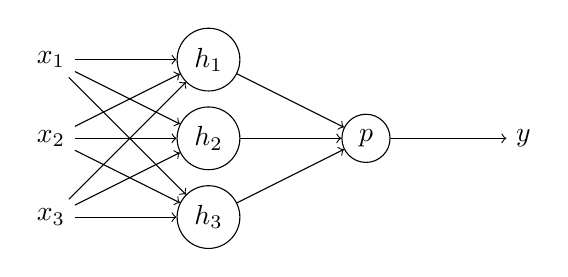
\begin{tikzpicture}[main/.style = {draw, circle}]
        \node (1) at (0,0) {$x_1$};
        \node (2) at (0,-1) {$x_2$};
        \node (3) at (0,-2) {$x_3$};
        \node[main] (4) at (2,0) {$h_1$};
        \node[main] (5) at (2,-1) {$h_2$};
        \node[main] (6) at (2,-2) {$h_3$};
        \node[main] (7) at (4,-1) {$p$};
        \node (8) at (6,-1) {$y$};
        \draw[->] (1) -- (4);
        \draw[->] (1) -- (5);
        \draw[->] (1) -- (6);
        \draw[->] (2) -- (4);
        \draw[->] (2) -- (5);
        \draw[->] (2) -- (6);
        \draw[->] (3) -- (4);
        \draw[->] (3) -- (5);
        \draw[->] (3) -- (6);
        \draw[->] (4) -- (7);
        \draw[->] (5) -- (7);
        \draw[->] (6) -- (7); 
        \draw[->] (7) -- (8);
    \end{tikzpicture}
    \caption{Ein Perzeptron mit drei Eingaben, drei versteckten Neuronen und einem Ausgabeneuron.}
\end{figure}

\Citeauthor{Rosenblatt1958} verkettete schon mehrere Perzeptronen zu einem mehrschichtigen Perzeptron , das in der Lage ist, nicht-lineare binäre Funktionen zu berechnen.
Dabei wird die Ausgabe eines Neurons als Eingabe für ein Neuron in einer darauf folgenden Schicht verwendet, wie in \ref{fig:perzeptron} zu sehen ist.
Ersetzt man die Sprungfunktion auch noch durch eine stetige Funktion, ist es nicht nur möglich auch stetige Funktionen zu berechnen.
Es lassen sich sogar alle stetigen Funktionen berechnen, deren Bildraum Teil des n-dimensionalen Hyperwürfel ist, wenn das mehrschichtige Perzeptron genügend Neuronen enthält \cite{Amari1967, Cybenko1989}.
Da diese Einschränkung sehr schwach ist, wird dies als universelle Approximationseigenschaft bezeichnet und ist ein wichtiger Grund, warum KNNs so vielfältig einsetzbar sind.

Heute werden KNNs dieser Art als Feedforward-Netzwerke bezeichnet.
Ist die Aktivierungsfunktion der Neuronen differenzierbar, können die Gewichte des Netzwerks durch das sogenannte Gradientenabstiegsverfahren optimiert werden.
Dieser Algorithmus wurde schon in den 1960er Jahren benutzt um die Gewichte für KNNs zu optimieren \cite{Amari1967}.
Er wurde aber erst in den 1980er Jahren populär, als es möglich wurde, ihn auf Computern effizient mit dem Backpropagation-Verfahren auszuführen \cite{Rumelhart1986}.
Um die Gewichte des Netzwerks zu optimieren, wird eine Kostenfunktion definiert, die die Differenz zwischen den Ausgaben des Netzwerks und den gewünschten Ausgaben bei gegebenen Trainingsbeispielen misst.
Dann wird ausgehend von einer Initialisierung der Gewichte die Kostenfunktion durch Anpassung der Gewichte minimiert.
Gleichzeitig für jedes Gewicht $w$ wird die partielle Ableitung der Kostenfunktion $C(w)$ nach dem Gewicht berechnet und das Gewicht in die entgegengesetzte Richtung der Ableitung verschoben:

$$
w \leftarrow w - \alpha \frac{\partial C(w)}{\partial w}
$$

Die Lernrate $\alpha$ ist eine positive Konstante, die die Schrittweite bestimmt.
Der Prozess wird so lange wiederholt, bis die Kostenfunktion einen akzeptablen Wert erreicht hat.

Das Backpropagation-Verfahren ist prinzipiell die Anwendung der Kettenregel der Differentialrechnung auf die Kostenfunktion um die partiellen Ableitungen zu berechnen.
All dies scheint auf den ersten Blick sehr einfach, aber in der Praxis gibt es viele Herausforderungen, die es zu bewältigen gilt.

Neben der theoretischen Einschränkung, dass das Gradientenabstiegsverfahren nur das Finden lokaler Minima der Kostenfunktion garantiert, gibt es auch praktische Einschränkungen.
In den Anfängen des maschinellen Lernens war es nicht praktikabel, die partiellen Ableitungen der Kostenfunktion für große Netze zu berechnen, weil es an Rechenleistung fehlte.
Es ist außerdem wahrscheinlich, dass aufgrund der universellen Approximationseigenschaft für KNNs mit nur einer Zwischenschicht viel mit nicht optimalen Netzwerkarchitekturen experimentiert wurde.
Deshalb ist es nicht verwunderlich, dass KNNs ab den 1990er Jahren weniger Aufmerksamkeit bekamen, als die Erwartungen nicht erfüllt wurden, während andere Methoden des maschinellen Lernens, wie Support Vector Machines, erfolgreich waren \cite{Schmidhuber2015}.
Erst in den 2010er Jahren, als die Rechenleistung und die Datenmengen groß genug wurden, um tiefe Netzwerke mit mehr Schichten zu trainieren, begannen KNNs langsam ihren heutigen Status\footnote{Der Ruf von KNNs als Panakeia ist mehr als zweifelhaft, denn \glqq es gibt nichts umsonst\grqq{} (\textit{"There is no such thing as a free lunch"}) \cite{NoFreeLunch}.} zu erreichen \cite{Schmidhuber2015}.

Bevor wir uns den LLMs zuwenden, will ich noch auf andere KNN-Architekturen eingehen, die für die Verarbeitung von natürlicher Sprache eingesetzt wurden.
Natürliche Sprache liegt immer in Form von Sequenzen vor (Sätze, Wörter, Phoneme, Buchstaben, etc.).
Um diese Sequenzen zu verarbeiten, wurden spezielle KNN-Architekturen entwickelt.
Ein solches KNN ist das rekurrente neuronale Netzwerk (RNN), das für die Verarbeitung von Sequenzen eingesetzt wird \cite{bidirectional_rnn}.
Rekurrente neuronale Netze funktionieren prinzipiell wie Feedforward-Netzwerke, aber sie haben auch eine Rückkopplungsschleife, die es ihnen ermöglicht, Informationen über die Zeit zu speichern.
Dafür wird das Netzwerk um eine zusätzliche Ein- und Ausgabe erweitert, die den versteckten Zustand des Netzwerks repräsentiert.
Diese Ausgabe wird dann als zusätzliche Eingabe in den nächsten Berechnungsschritt gegeben.
Dadurch können RNNs beliebig lange Sequenzen verarbeiten und das \glqq aufgefaltete\grqq{} Netz, wie in \ref{fig:rnn} dargestellt, kann als großes nicht-rekurrentes Netzwerk betrachtet und trainiert werden.
Damit ein RNN in der Lage ist, Abhängigkeiten von beliebigen Teilen der Eingabesequenz auf die ersten Ausgaben zu erfassen, müssen entweder verdeckte Zustände in beide Richtungen übertragen werden (bidirektionale RNNs) oder die Ausgabe wird erst nach der gesamten Eingabesequenz berechnet \cite{bidirectional_rnn}.

\begin{figure}
\label{fig:rnn}
\centering
%tkz-graph of the block structure of an RNN
\begin{tikzpicture}[main/.style = {draw}]

    % instances of the RNN
    \node[main] (1) at (0,0) {$R$};
    \node[main, right=of 1] (2) {$R$};
    \node[right=of 2] (3) {$\cdots$};
    \node[main, right=of 3] (4) {$R$};
    \node[main, right=of 4] (5) {$R$};

    % Input nodes
    \node[below=of 1] (6) {$x_1$};
    \node[below=of 2] (7) {$x_2$};
    \node[below=of 4] (8) {$x_t$};
    \node[below=of 5] (9) {$x_{t+1}$};

    % Output nodes
    \node[above=of 1] (10) {$y_1$};
    \node[above=of 2] (11) {$y_2$};
    \node[above=of 4] (12) {$y_t$};
    \node[above=of 5] (13) {$y_{t+1}$};

    % Initial state
    \node[left=of 1] (14) {$h_0$};

    % Connections between the instances
    \draw[->] (14) -- (1);
    \draw[->] (1) -- (2);
    \draw[->] (2) -- (3);
    \draw[->] (3) -- (4);
    \draw[->] (4) -- (5);

    % Connections between the input and the instances
    \draw[->] (6) -- (1);
    \draw[->] (7) -- (2);
    \draw[->] (8) -- (4);
    \draw[->] (9) -- (5);

    % Connections between the instances and the output
    \draw[->] (1) -- (10);
    \draw[->] (2) -- (11);
    \draw[->] (4) -- (12);
    \draw[->] (5) -- (13);
\end{tikzpicture}
\caption{Ein \glqq aufgefaltetes\grqq{} rekurrentes KNN. Die Eingaben $x_i$ und die Ausgaben $y_i$ sind die Elemente der Eingabe- und Ausgabesequenzen. $h_0$ ist der Anfangszustand des Netzwerks und $R$ ist das rekurrente KNN.}
\end{figure}

Gerade wenn man die Ausgabe erst nach der gesamten Eingabesequenz berechnet, kann es zu Problemen kommen, wenn die Eingabesequenz lang ist \cite{vanishing_gradients}.
Bei der Gradienten für das Training in den Termen, die Abhängigkeiten zwischen weit auseinander liegenden Teilen der Eingabe- und Ausgabe repräsentieren, werden die partiellen Ableitungen der Aktivierungsfunktionen immer wieder multipliziert.
Das führt bei sigmoidalen Aktivierungsfunktionen dazu, dass diese Terme sehr schnell gegen Null konvergieren und das Netzwerk keine Abhängigkeiten über längere Distanzen lernen kann.
Das Problem wurde als \glqq verschwindende Gradienten\grqq{} bezeichnet und ist ein Grund, warum RNNs in der Praxis oft nicht gut funktionieren.

Es gibt verschiedene Ansätze, um das Problem der verschwindenden Gradienten zu mildern.
Dazu gehören spezielle Initialisierungen der Gewichte, andere Aktivierungsfunktionen und die Verwendung von Batch-Normalisierung \cite{vanishing_gradients}.
Batch-Normalisierung, welches auch in den von dieser Arbeit eingesetzten Modellen benutzt wird, ist heute ein Standardansatz, bei der die Ausgaben jeder Schicht so skaliert werden, dass sie einen Mittelwert von Null und eine Standardabweichung von Eins haben \cite{batch_normalization}.
Warum Batch-Normalization so gut gegen das Problem der verschwindenden Gradienten hilft ist nicht vollständig verstanden, zumindest gibt es verschiedene Erklärungsansätze \cite{batch_normalization,batch_norm_reason_1,batch_norm_reason_2}.

Vor Batch-Normalization war es aber auch schon möglich, RNNs aus Long Short-Term Memory (LSTM) Zellen zu modellieren, die speziell dafür entwickelt wurden, Abhängigkeiten über längere Distanzen zu lernen \cite{lstm}.
LSTM-Zellen sind eine Abkehr von den einfachen Feedforward-Schichten.
Ihre Struktur ist komplexer und so konstruiert, dass es zusätzlich zu dem versteckten Zustand, den es auch in einfachen RNNs gibt, einen Zellzustand gibt, der nicht in jedem Schritt mit einer Aktivierungsfunktion verkleinert wird.
Dadurch kann der Gradient ungehindert durch das Netzwerk \glqq fließen\grqq{} und Abhängigkeiten über längere Distanzen gelernt werden.
Der Zellzustand wird durch drei sogenannte \glqq Gatter\grqq{} gesteuert, die die Information im Zellzustand aktualisieren, löschen oder ausgeben.
Eine schematische Darstellung einer LSTM-Zelle ist in \ref{fig:lstm} zu sehen.

\begin{figure}
\label{fig:lstm}
\centering
\newcommand*{\connectorH}[4][]{
  \draw[#1] (#3) -| ($(#3) !#2! (#4)$) |- (#4);
}
\newcommand*{\connectorV}[4][]{
  \draw[#1] (#3) |- ($(#3) !#2! (#4)$) -| (#4);
}
\begin{tikzpicture}[operator/.style = {draw, circle}, activation/.style = {draw}]
    \node (1) at (0,0) {$c_{t-1}$};
    \node[operator,right=2cm of 1] (2) {$\times$};
    \node[activation,below=2cm of 2] (3) {$\sigma$};
    \node[activation,right=of 3] (4) {$\sigma$};
    \node[activation,right=of 4] (5) {$\tanh$};
    \node[operator,below left=of 3] (9) {$\circ$};
    \node[activation,right=5.5cm of 9] (6) {$\sigma$};
    \node[operator,right=of 6] (7) {$\times$};
    \node[activation,above=1.5cm of 7] (8) {$\tanh$};
    \node[below=of 9] (10) {$x_i$};
    \node[left=of 9] (11) {$h_{t-1}$};
    \node[operator,above=0.7cm of 5] (12) {$\times$};
    \node[operator,right=2.6cm of 2] (13) {$+$};
    \node[right=5cm of 13] (14) {$c_t$};
    \node[above left=of 14] (15) {$h_t$};
    \node[right=2cm of 7] (16) {$h_t$};

    % connectors
    \draw[->] (1) -- (2);
    \draw[->] (3) -- (2);
    \draw[->] (6) -- (7);

    \draw[->] (11) -- (9);
    \draw[->] (10) -- (9);
    \draw[->] (9) -| (3);
    \draw[->] (9) -| (4);
    \draw[->] (9) -| (5);
    \draw[->] (9) -- (6);

    \draw[->] (4) |- (12);
    \draw[->] (5) -- (12);
    \draw[->] (2) -- (13);
    \draw[->] (12) -- (13);
    \draw[->] (13) -| (8);
    \draw[->] (8) -- (7);
    \draw[->] (7) -- (16);
    \draw[->] (7) -| (15);
    \draw[->] (13) -- (14);
\end{tikzpicture}
\caption{Eine schematische Darstellung einer LSTM-Zelle. Die Eingabe $x_i$, der versteckte Zustand $h_{t-1}$ und der vorherige Zellzustand $c_{t-1}$ werden in die Zelle gegeben. Der verdeckte Zustand $h_t$ ist gleichzeitig die Ausgabe der Zelle. $\circ$, $\sigma$ und $\tanh$ sind die Verkettung, Sigmoid- und Tangenshyperbolicus-Aktivierungsfunktionen.}
\end{figure}

Convolutionale neuronale Netze (CNNs) sind eine weitere wichtige Architektur von KNNs, die hauptsächlich für die Verarbeitung von Bildern und anderen zweidimensionalen Datenstrukturen benutzt wird \cite{neocognitron}.
Sie bestehen aus einer Reihe von Schichten, die aus Faltungsschichten, Pooling-Schichten und vollständig verbundenen Schichten bestehen.
Im Gegensatz zu rekurrenten Netzen haben sie eine feste Sichtweite, die durch die Größe der Faltungskerns bestimmt wird.
Deshalb werden CNNs eher selten für die Verarbeitung von natürlicher Sprache benutzt, aber es gibt Anwendungen, bei denen sie erfolgreich eingesetzt wurden \cite{tdnn}.


\section{Transformer: Ein Überblick}
\label{subsec:Foundations:Transformer}
Transformer \cite{transformers} sind eine Klasse von Deep-Learning-Modellen, die sich bei einer Vielzahl von Aufgaben der linguistischen Datenverarbeitung wie maschineller Übersetzung, Text\-er\-zeugung und Sprachmodellierung als äußerst effektiv erwiesen hat \cite{transformers,bert,FewShotLearners,gpt4}.
Sie basieren auf einer Architektur, die sich von herkömmlichen rekurrenten neuronalen Netzen (RNNs) und Convolutional Neural Networks (CNNs) unterscheidet.
In jedem Schritt der Verarbeitung wird die Eingabesequenz zu jeweils einem Ausgabetoken verarbeitet.
Durch wiederholte Anwendung kann so eine Sequenz von Ausgabetoken erzeugt werden.
Ein grundlegender Baustein eines Transformer-Modells ist der Self-Attention-Mechanismus, der es dem Modell ermöglicht, sich während der Kodierungs- und Dekodierungsphasen auf bestimmte Teile der Ein- und Ausgabesequenzen zu „konzentrieren“.
Er ist notwendig um Abhängigkeiten zwischen weit voneinander entfernten Teilen der Eingabe zu erfassen, was besonders wichtig für Aufgaben des Sprachverständnisses ist.
In einem Transformer-Modell wird die Eingabesequenz zunächst von einer Reihe von Kodierungsschichten verarbeitet, die jeweils aus einem Self-Attention-Modul und einem neuronalen Feedforward-Netzwerk bestehen.
Das Self-Attention-Modul berechnet eine Gewichtung der Aufmerksamkeit auf die Positionen in der Eingangssequenz, die verwendet wird, um den Einfluss dieser Eingabeteile auf das jeweils nächste Ausgabetoken zu vergrößern.
Nach den Kodierungsschichten wird die Ausgabesequenz durch eine Reihe von Dekodierungsschichten erzeugt, die im Gegensatz zu den Kodierungsschichten sowohl auf die Eingabesequenz als auch auf die zuvor erzeugten Ausgabesequenzen zugreifen.
Die Dekodierungsschichten ermöglichen es dem Modell, Ausgabesequenzen zu erzeugen, die von der Eingabesequenz und zuvor erzeugten Ausgabetokens abhängen.
Einer der Hauptunterschiede von Transformermodellen gegenüber den älteren RNNs ist, dass zwischen den einzelnen Berechnungsschritten kein Zustand mitgeführt wird.
Das hat zwei Vorteile: Dieser Zustand kann nicht „vergessen“ werden und da keine Abhängigkeiten zwischen den Trainingsschritten existieren kann das Modell besser parallel trainiert werden.

Insgesamt können Transformermodelle Eingaben und Ausgaben variabler Länge verarbeiten und lassen sich mit großen Datensätzen trainieren, wodurch sie sich gut für Aufgaben der linguistischen Datenverarbeitung eignen.
Transformer haben sich für eine Vielzahl von Aufgaben der linguistischen Datenverarbeitung zum State-of-the-Art-Ansatz entwickelt und sind nach wie vor ein aktives Forschungsgebiet.
Zu den jüngeren Fortschritten gehören Techniken für das Training immer größerer Transformermodelle auf riesigen Datensätzen:
Zu den bekanntesten Transformermodellen gehören BERT \cite{bert}, GPT-3 \cite{FewShotLearners} und GPT-4 \cite{gpt4}, die sich vor allem in ihrer Größe, aber mutmaßlich nicht grundlegend in ihren Architekturen unterscheiden \footnote{Im Fall von GPT-4, werden auch Bilder als Teil der Eingabe akzeptiert. Die genaue Architektur von GPT-4 ist nicht öffentlich bekannt.}.
Als Bezeichnung für diese Modelle hat sich der Begriff Large Language Model (LLM) etabliert.

\section{Große Sprachmodelle und ihre Anwendungen in der Softwareentwicklung}
\label{subsec:Foundations:LLM}


\todo{Komplett überarbeiten oder löschen}

Large language models like GPT-3 can be used task-agnostically because they are trained on vast amounts of text data in an unsupervised manner. During training, the model learns to understand the underlying patterns and relationships in language, allowing it to generate coherent and contextually appropriate responses to a wide range of tasks without the need for task-specific training data.
One key advantage of these models is their massive size, with GPT-3 containing 175 billion parameters.
This allows them to capture a vast amount of linguistic knowledge and context.
Because these models have been trained on such a large and diverse corpus of text, they are able to learn and generalize from patterns and relationships that are common across many different types of language use. This allows them to perform well on a wide variety of natural language processing tasks, such as language translation, sentiment analysis, and question answering, among others.
The sheer number of parameters used in these models allows them to capture a wide range of linguistic features, from simple grammatical structures to more complex semantic relationships. By leveraging this large amount of training data and parameter space, these models are able to learn to represent language in a highly nuanced and contextually appropriate way, allowing them to perform well on a wide range of tasks without the need for additional training.
Furthermore, GPT-3 has shown impressive capabilities in generating source code for computer programs, including JavaScript, Python, and SQL. As a language model trained on a massive amount of code and natural language data, ChatGPT can also generate source code with a high degree of accuracy and efficiency, making it a valuable tool for software development and automation tasks.
As such LLMs appear to be adequate to process both the structured representation of an application’s GUI, as well as natural language test cases, and provide a description of what action to follow next.

\chapter{Stand der Technik}
\label{ch:RelatedWork}

Ein verbreiteter Ansatz für das automatische Testen von Webanwendungen ohne hartkodierte Fehlerbedingungen ist das sogenannte Monkey-Testing.
Dabei werden zufällige Benutzerinteraktionen simuliert und beobachtet, ob die Anwendung abstürzt.
Dieser Ansatz ist einfach zu implementieren und kann auf jede Webanwendung angewendet werden, unabhängig von ihrer Struktur \cite{monkey_testing}.

Aufbauend auf Monkey-Testing gibt es viele Ansätze mit der Idee, Algorithmen zu entwickeln, die die zu testende Anwendung effizienter erkunden.
TESTAR, ein Werkzeug für Monkey-Testing, enthält auch einen Algorithmus, der den Suchraum auf „interessante“ Pfade einschränken soll.
Dafür wird eine anwendungsspezifische Prolog Wissendatenbank verwendet, die relevante Benutzeraktionen aus dem Anwendungszustand ableitet.
Aus diesen wird mittels Q-Learning ein Modell trainiert, das alle Anwendungszustände effizient zu erforschen versucht \cite{testar-q-learning}.
Eskonen et al. verwenden bildbasiertes Deep Reinforcement Learning, um zu imitieren, wie Menschen die zu testende Anwendung erkunden \cite{deep_reinforcement_exploring}.
Auf ähnliche Weise nutzen Saber et al. Computer Vision, um Anwendungszustände und Interaktionselemente aus Screenshots zu extrahieren, und verwenden dann Deep Q-Learning, um alle Anwendungszustände effizient zu erforschen \cite{saber_testing}. 
%Diese Ansätze machen zwar menschliche Interaktion überflüssig und sind auf jede GUI-basierte Anwendung anwendbar, ermöglichen aber nicht die automatische Abarbeitung von natürlichsprachlichen Designer-Testfällen.
Harris et al. schlagen DRIFT vor, ein Framework zur Navigation durch eine zu testende Anwendung, bei der zuvor spezifizierte Softwarefunktionen ausgelöst werden sollen \cite{harries2020drift}.
DRIFT arbeitet mit einer symbolischen Darstellung der Benutzeroberfläche und verwendet Q-Learning mit Graph Neural Networks.
Dieser Prozess setzt jedoch die Beobachtung von Funktionsaufrufen der zu testenden Anwendung voraus; die Definition von Tests erfordert technische Kenntnisse über die Interna der Anwendung.
Khaliq et al. verwenden ein ähnliches System wie das in dieser Arbeit vorgeschlagene: Sie übergeben kurze textuelle Beschreibungen der Benutzeroberfläche an ein LLM, das eine Sequenz von Benutzeraktionen generiert, die von diesem Zustand aus zu verfolgen sind \cite{transformers_exploratory}.
Neuere LLMs mit längereren maximalen Eingaben erlauben es jetzt aber, die vollständige Repräsentation der GUI in der Eingabe zu verwenden.

Diese Arbeit folgt dem Ansatz von \Citeauthor{GPT3Testing}, eine strukturierte Darstellung der Benutzeroberfläche der zu testenden Anwendung zusammen mit einer natürlichsprachlichen Testbeschreibung als Eingabe für ein LLM-Modell zu verwenden \cite{GPT3Testing}.
Das LLM generiert dann eine Benutzerinteraktion, die automatisch in der Anwendung ausgeführt wird.
Sie evaluieren ihren Ansatz anhand einer sehr einfachen Anwendung, die aus einer Ansicht mit Knöpfen besteht und einer Vielzahl von Testbeschreibungen.
Diese Arbeit zielt darauf ab, eine automatisierte Pipeline zu entwickeln und zu validieren, die den gleichen Ansatz für allgemeine GUI-basierte Webanwendungen mit HTML verwendet.

Meines Wissens nach gibt es keine anderen Arbeiten, die LLMs für das automatisierte Testen von Webanwendungen verwenden.
In neueren Literaturübersichten wird die linguistische Sprachverarbeitung zwar als Werkzeug für das Testen von Software aufgeführt, jedoch nicht für das Generieren von Benutzerinteraktionen \cite{implementation_verma_2023, machine_fontes_2021}.

% Das hier in anderes Kapitel???? Nein, das ist hier richtig
Scheinbar notwendig für diese Anwendung ist die Fähigkeit des LLMs, die GUI und Zustände der zu testenden Anwendung zu verstehen und zu navigieren.
Zu dieser Navigation ist die Repräsentation der GUI als HTML-Dokument, einer Baumstruktur, von Bedeutung, und der Zustandsgraph, der sich aus den möglichen Benutzerinteraktionen (Kanten) und Zuständen der Anwendung ergibt (Knoten).
Ergebnisse der Kognitionswissenschaft legen allerdings nahe, dass zum Verständnis solcher Graphen eine Art von räumlichem Verständnis erforderlich ist \cite{what_is_a_cognitive_map}, das bisher bei LLMs scheinbar nicht vorhanden ist:
Die Sprachmodelle konnten Fragen, die ein Verständnis der Navigation in einfachen Raumplänen erforderten, nicht korrekt beantworten \cite{cogmaps_llm}.
Erschwerend kommt hinzu, dass der Zustandsgraph der Webanwendungen in dieser Anwendung nicht explizit gegeben ist, sondern vom LLM aus den Interaktionen mit der Webanwendung abgeleitet werden müsste.

Einen komplett anderen Ansatz bieten Tsung et al.
Sie stellen einen Arbeitsablauf vor, der auf der Spezifikation von Testskripten in einer strukturierten, für den Menschen lesbaren Sprache basiert, die auch Bilder enthält \cite{tsung}.
Diese Skripte sind mit sehr wenig technischem Wissen verständlich und müssen nicht geändert werden, solange die visuellen Elemente der Benutzeroberfläche gleich bleiben.
Auch wenn keine natürliche Sprache verwendet wird und Änderungen an der Benutzeroberfläche immer noch Änderungen am Skript erforderlich machen können, werden einige Nachteile regulärer Testskripte beseitigt.


\chapter{Versuchsaufbau}
\label{ch:ExperimentalSetup}

Nachdem die Arbeit von \Citeauthor{GPT3Testing} nur an einem einfachen Taschenrechner getestet wurde, stellt sich die Frage, welche Art von Anwendung für eine ausführlichere Evaluation des Ansatzes geeignet ist.
Meiner Meinung nach sollte die Anwendung mindestens folgende Eigenschaften haben:

\begin{enumerate}
    \item
        Die Anwendung sollte praxisrelevant sein, idealerweise sollte sie sich nicht grundlegend von einer realen Anwendung unterscheiden.
    \item
        Die Anwendung sollte eine Vielzahl unterschiedlicher Interaktionselemente ent\-hal\-ten, die getestet werden können. 
        Sie sollte zumindest Hyperlinks, Knöpfe und Textfelder enthalten.
    \item
        Die Anwendung sollte transaktionale Arbeitsabläufe enthalten.
        Das bedeutet, dass der Benutzer eine Reihe von Interaktionen ausführen muss, um eine bestimmte Aktion auszuführen.
    \item
        Die Anwendung sollte Validierungslogik enthalten: Die Benutzereingaben sollten auf Korrektheit überprüft werden und die Anwendung sollte den Benutzer auffordern, fehlerhafte Eingaben zu korrigieren.
        Dadurch ist der Tester gezwungen, auf Feedback der Anwendung zu reagieren, um eine bestimmte Interaktion auszuführen.
    \item
        Der Zustandsgraph der Anwendung sollte einen hohen Verzweigungsgrad haben.
        Der Verzweigungsgrad eines Graphen ist ein Maß für die Komplexität des Graphen.
        Er wird in endlichen Graphen als die Anzahl der Kanten geteilt durch die Anzahl der Knoten definiert.
        Im Kontext eines GUI bedeutet das, dass es viele mögliche Benutzeraktionen gibt, die zu verschiedenen Anwendungszuständen führen.
    \item 
        Die Anwendung sollte Open-Source sein, um die Reproduzierbarkeit der Ergebnisse zu gewährleisten.
        Sie sollte auch unter einer Lizenz stehen, die kompatibel mit der Veröffentlichung dieser Arbeit ist, das heißt kompatibel mit der GNU General Public License, Version 3.
    \item Schließlich ist eine textuelle Repräsentation der GUI der Anwendung notwendig, um sie dem LLM zu übergeben.
\end{enumerate}

Die Eigenschaften 1 bis 5 sind notwendig, um die Resultate der Evaluation auf möglichst viele reale Anwendungen übertragen zu können.
Abbildung \ref{fig:sad_monkey} zeigt, dass Eigenschaften 3 bis 5 außerdem interessant sind, weil sie zusammen naives Monkey-Testing ineffizient machen und somit die Fähigkeiten des LLMs auf die Probe stellen.

\begin{figure}
    \centering
    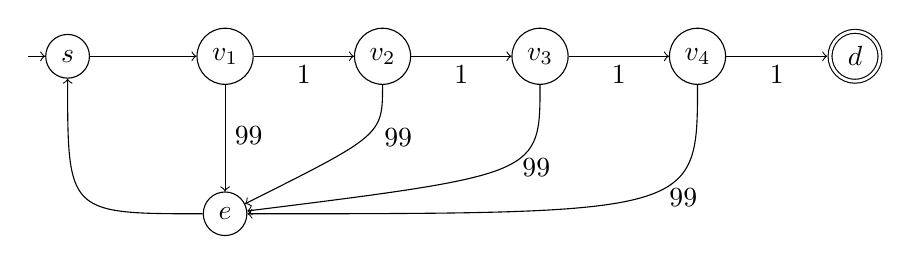
\begin{tikzpicture}[main/.style = {draw, circle},double_border/.style={draw, double, double distance=1pt,outer sep=1pt}] 
        \node[main] (1) at (0,0) {$s$};
        \node[main] (2) at (2, 0) {$v_1$};
        \node[main] (3) at (4, 0){$v_2$};
        \node[main] (4) at (6, 0) {$v_3$};
        \node[main] (5) at (8, 0) {$v_4$};
        \node[main,double_border] (6) at (10, 0) {$d$};
        \node[main] (7) at (2, -2) {$e$};
        \draw[->] (1) -- (2);
        \draw[->] (2) -- node[below] {$1$} (3);
        \draw[->] (3) -- node[below] {$1$} (4);
        \draw[->] (4) -- node[below] {$1$} (5);
        \draw[->] (5) -- node[below] {$1$} (6);
        \draw[->] (5) .. controls +(down:2) .. node[align=right,right] {\ \ $99$} (7);
        \draw[->] (4) .. controls +(down:1.5) .. node[right] {\ $99$} (7);
        \draw[->] (3) .. controls +(down:1) .. node[right] {\ $99$} (7);
        \draw[->] (2) .. controls +(down:1) .. node[right] {$99$} (7);
        \draw[->] (7) .. controls +(left:2) ..  (1);
        \draw[->] (-0.5,0) -- (1);
    \end{tikzpicture} 
    \caption{Zustandsgraph einer fiktiven Anwendung mit Validierung, einem transaktionalen Arbeitsablauf und einem hohen Verzweigungsgrad. $s$ ist der Startzustand, $d$ ist der Zielzustand, $e$ ist ein Fehlerzustand. Die Zahlen an den Kanten stehen für die Anzahl der möglichen Benutzerinteraktionen, die den Zustandsübergang auslösen. Die Wahrscheinlichkeit, dass ein Monkey-Tester den Zielzustand und nicht erneut den Startzustand erreicht, ist lediglich eins in hundert Millionen.}
    \label{fig:sad_monkey}
\end{figure}

Eine Art von Anwendung, die diese Anforderungen erfüllen kann, sind Webshops:
Webshops enthalten eine Vielzahl von Interaktionselementen, wie Produktlisten, Warenkörbe und Kassenprozesse.
Sie enthalten transaktionale Arbeitsabläufe, wie das Hinzufügen von Produkten zum Warenkorb gefolgt von einer Bestellung.
Sie enthalten Validierungslogik, zum Beispiel bei dem Ausfüllen von Adressfeldern.
Sie haben einen hohen Verzweigungsgrad, da es viele verschiedene Produkte gibt, die zu verschiedenen Anwendungszuständen führen.
Außerdem sind sie praxisrelevant: Der Marktanteil von E-Commerce ist groß und wächst weiter.
\footnote{
Der Anteil von E-Commerce am Einzelhandelsumsatz in den USA betrug im Quartal 1, 2023 15,6\%. U.S. Bureau of the Census über FRED, Federal Reserve Bank of St. Louis. \url{https://fred.stlouisfed.org/series/ECOMPCTSA}}
Und erfreulicherweise sind ihre GUIs in der Regel Webseiten, sodass die textuelle Repräsentation ihrer GUI, das HTML-Dokument, direkt verfügbar ist.

Um eine geeignete Anwendung zu finden, habe ich eine Reihe von Open-Source-Projekten durchsucht, die als Webshop-Software oder Template für solche vermarktet werden.
Eine Auswahl dieser Projekte ist in Abbildung \ref{tab:webshop_projects} aufgeführt.

\begin{figure}[h]
    \begin{minipage}[c]{\textwidth}
        \centering
        {
            \scriptsize
            \begin{tabular}{ | l | l | l | l | l |}
                \hline
                \textbf{Projekt} & \textbf{Letzter Commit} & \textbf{Lizenz} & \textbf{Technologie} & \textbf{Vermerk} \\ \hline
                Online Shopping Cart\footnote{\url{https://github.com/shashirajraja/shopping-cart}} & Mai 23 & Apache 2 & Java, Servlets, JSP, SQL & Demonstrationszweck \\ \hline
                LifestyleStore\footnote{\url{https://github.com/sajalagrawal/LifestyleStore}} & August 20 & - & PHP, SQL & Lernzweck \\ \hline
                Your Online Shop\footnote{\url{https://github.com/petazeta/youronlineshop}} & Dezember 22 & custom & Node.js, MongoDB & - \\ \hline
                Ecommerce-Website\footnote{\url{https://github.com/winston-dsouza/ecommerce-website}} & Februar 20 & MIT & PHP, SQL & keine transaktionalen Workflows \\ \hline
                Book-Hub\footnote{\url{https://github.com/amberkakkar01/Book-Hub}} & August 21 & - & HTML & statisches HTML \\ \hline
                online-shopping-site\footnote{\url{https://github.com/dinushchathurya/online-shopping-site}} & Mai 19 & GPLv3 & JavaScript & ohne Server \\ \hline
                Online-Fashion-Store\footnote{\url{https://github.com/RazaRizvii/Online-Fashion-Store}} & Dezember 22 & - & JavaScript & ohne Server \\ \hline
                online-shopping-website\footnote{\url{https://github.com/nsk1512/online-shopping-website}} & Dezember 19 & - & Node.js, MongoDB & - \\ \hline
                Ketra-Mart\footnote{\url{https://github.com/Prajwal100/ketra-mart-free}} & Juni 23 & MIT & ? & Quellcode nur gegen Zahlung \\ \hline
                Shuup\footnote{\url{https://github.com/shuup/shuup}} & August 21 & OSL & Python, SQL & Kommerziell, Multi-Vendor \\ \hline
                EverShop\footnote{\url{https://github.com/evershopcommerce/evershop}} & September 23 & GPLv3 & Node.js, SQL & - \\ \hline
                Hayroo\footnote{\url{https://github.com/hasan-py/MERN_Stack_Project_Ecommerce_Hayroo}} & May 23 & - & Node.js, MongoDB & - \\ \hline
            \end{tabular}
        }
    \end{minipage}
    \caption{Open-source Webshop Projekte, die für die Verwendung in dieser Arbeit gesichtet wurden.}
    \label{tab:webshop_projects}
\end{figure}

Die meisten dieser Projekte sind nicht für die Verwendung in dieser Arbeit geeignet, da sie entweder nicht transaktional sind oder keine passende Lizenz haben.
\textit{EverShop} und \textit{Shuup} erfüllen zwar alle Anforderungen, sind aber so komplex und umfangreich, dass ein maßgeblicher Teil der Arbeit darin bestehen würde, die Anwendung zu verstehen und zu modifizieren, um sie für die Evaluation des Ansatzes zu verwenden.

\textit{online-shopping-website} hingegen ist streng genommen nicht für den praktischen Einsatz gedacht, erfüllt aber fast alle Anforderungen und ist klein und simpel.
Nur eine Möglichkeit zur Kaufabwicklung mit einer validierten Eingabemaske fehlt, welche aber mit vertretbarem Aufwand hinzugefügt werden kann.
Deshalb wurde entschieden, eine eigene Anwendung auf Basis von \textit{online-shopping-website} zu entwickeln, die alle Anforderungen erfüllt und gleichzeitig einfach genug ist, um sie in der verfügbaren Zeit zu evaluieren.

\section{Forschungsfragen}

\todo{Keine Orakel, nur Interaktionen}

\begin{enumerate}
    \item Can LLMs understand HTML?
    \item Feasibility of the approach
    \item Do you need the whole document? / Advantage of “stripped tree”
    \item Flakiness > Repeats necessary / how many?
    \item Optional: Possibility and Accuracy of validation
    \item Optional: Impact of prompt engineering?
\end{enumerate}

\section{Getestete Anwendung}

Um die Methode des automatisierten Testens von Webanwendungen mit LLMs zu evaluieren, habe ich eine eigene Anwendung entwickelt, die als Test\-anwendung dient.
Diese Testanwendung ist ein Webshop, in dem Benutzer mit verschiedenen Elementen interagieren können, wie Produktlisten für verschiedene Produktkategorien, einem Warenkorb und dem Kassenprozess.

Als Grundlage für die Testanwendung dient das Open-Source Projekt \textit{online-shopping-website} \footnote{\url{https://github.com/nsk1512/online-shopping-website}}.
\textit{online-shopping-website} enthält bereits eine Startseite, Produktlisten und einen Warenkorb.
Die Anwendung ist in JavaScript geschrieben und benötigt keine externen Abhängigkeiten, Server oder Datenbanken.
Für diese Arbeit habe ich die Anwendung unter Verwendung der Bibliothek \textit{react}\footnote{\url{https://react.dev/}} neu implementiert und um eine Kassenfunktionalität, Validierungslogik und eine Bestellbestätigungsseite erweitert.
Mit diesen Erweiterungen erfüllt die Anwendung alle Anforderungen, die am Anfang dieses Kapitels aufgeführt sind.

\todo{Das hier genauer, vllt. über Benutztererfahrung? Startseite -> Produktliste -> Warenkorb -> Kasse -> Bestellbestätigung, subsubsection / Absatz / itemize, Anforderungen werden alle erfüllt!}

Die Webseite ist jetzt wie folgt aufgebaut:
Es gibt vier verschiedene Seiten, die der Benutzer besuchen kann: Die Startseite, die Produktlisten für verschiedene Produktkategorien, die Kasse und die Bestellbestätigungsseite.
Diese sind in Abbildung \ref{fig:online-shopping-website} dargestellt.
Jede Seite enthält eine Titelleiste mit einem aufklappbaren Menü, das den Benutzer zu den anderen Seiten führt und eine aufklappbare Warenkorbansicht.
Die Produktlisten und die Startseite enthalten Bilder, Namen und Preise der Produkte sowie eine Schaltfläche, um das Produkt zum Warenkorb hinzuzufügen.
Ursprünglich wurde der Knopf nur angezeigt, wenn der Benutzer mit der Maus über das Produktbild fährt, aber das wurde geändert, da das zu Probelemen mit der Extraktion von Benutzerinteraktionen führte.
Die Startseite enthält ausgewählte Produkte aus verschiedenen Kategorien und eine Schaltfläche, um zu einer hervorgehobenen Produktkategorie zu gelangen.
In dem aufklappbaren Warenkorb lassen sich die Produkte entfernen, die Anzahl der Produkte ändern und es gibt eine Schaltfläche, um zur Kasse zu gelangen.
In der Kasse gibt es eine Bestellübersicht, dort gibt der Benutzer seine Adresse und Zahlungsdaten ein und bestätigt die Bestellung.
Daraufhin werden die Benutzereingaben auf Vollständigkeit und korrekte Form validiert.
Falls sie korrekt sind, gelangt der Nutzer zur Bestellbestätigungsseite, sonst wird er aufgefordert, die Eingaben entsprechend zu korrigieren.

\begin{figure}
    \centering
    \begin{subfigure}[b]{0.32\textwidth}
        \centering
        
\includegraphics[width=\textwidth]{pictures/Start.png}
        \caption{Startseite}
        \label{fig:online-shopping-website-start}
    \end{subfigure}
    \hfill
    \begin{subfigure}[b]{0.32\textwidth}
        \centering
        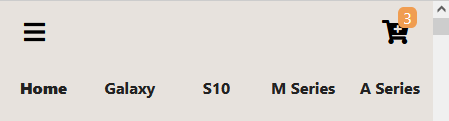
\includegraphics[width=\textwidth]{pictures/Leiste.png}
        \caption{auf\-ge\-klappte Titelleiste}
        \label{fig:online-shopping-website-menu}
    \end{subfigure}
    \hfill
    \begin{subfigure}[b]{0.32\textwidth}
        \centering
        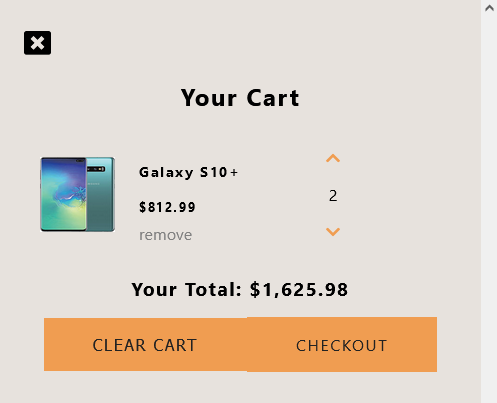
\includegraphics[width=\textwidth]{pictures/Cart.png}
        \caption{Warenkorb}
        \label{fig:online-shopping-website-cart}
    \end{subfigure}
    
    % New row
    \begin{subfigure}[b]{0.9\textwidth}
        \centering
        
\includegraphics[width=\textwidth]{pictures/Products_Half.png}
        \caption{Produktliste}
        \label{fig:online-shopping-website-product-list}
    \end{subfigure}
    \begin{subfigure}[b]{0.9\textwidth}
        \centering
        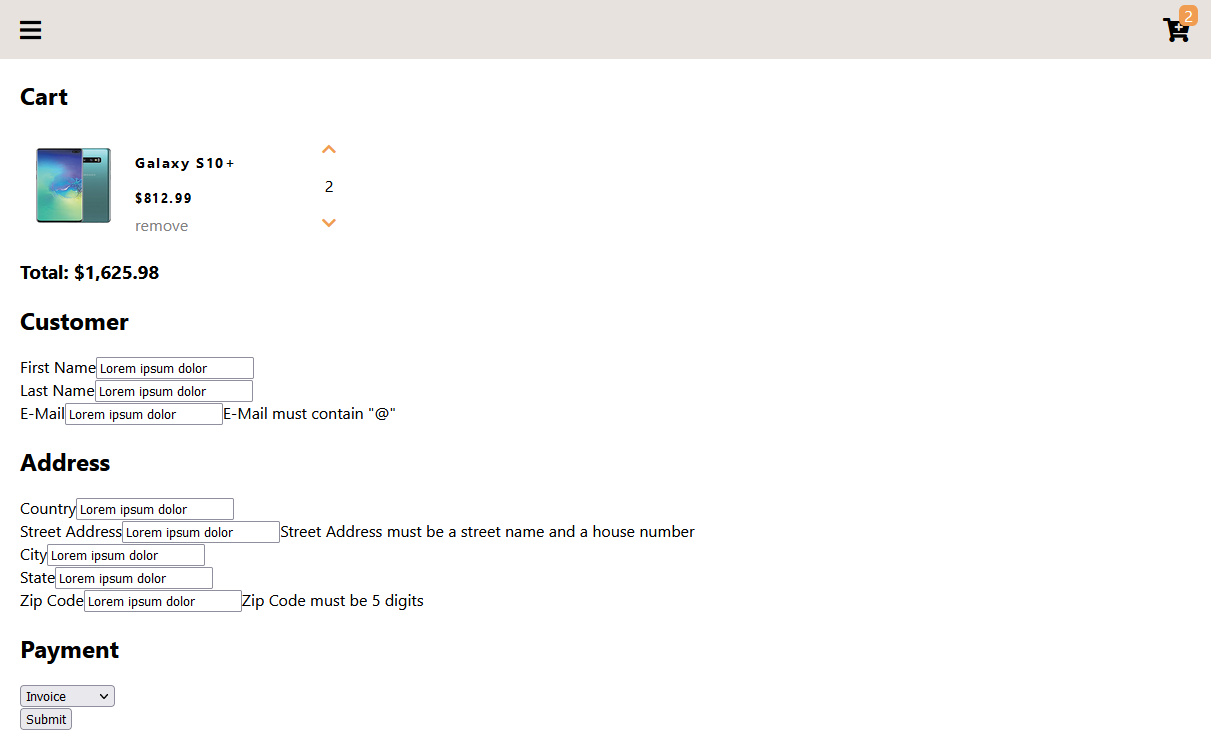
\includegraphics[width=\textwidth]{pictures/Checkout.png}
        \caption{Kasse}
        \label{fig:online-shopping-website-checkout}
    \end{subfigure}

    \caption{Screenshots der Testanwendung}
    \label{fig:online-shopping-website}
\end{figure}

\subsection*{Implementierung}

\textit{online-shopping-website}, auf dem die Testanwendung basiert, ist in JavaScript geschrieben und verwendet keine externen Abhängigkeiten, Server oder Datenbanken.
Die Anwendung besteht aus einer HTML-Datei, die die Struktur der Webseite definiert, einer JSON-Datei in der die Produkte gespeichert sind und einer JavaScript-Datei, die die Interaktionen der Benutzer mit der Webseite steuert.
Die HTML-Datei definiert statische Elemente der Webseite, wie die Titelleiste und das Overlay für den Warenkorb.
Alle andern Elemente werden dynamisch von der JavaScript-Datei generiert.
Dieser Ansatz ist für das \textit{online-shopping-website} gerade ausreichend, aber würde für eine größere Anwendung schnell unübersichtlich werden.
Deshalb habe ich die Anwendung in \textit{react} neu implementiert.
\textit{react} ist eine Bibliothek, die es erlaubt, Webseiten aus wiederverwendbaren Komponenten zu bauen.
Komponenten sind in \textit{react} Funktionen höherer Ordnung, die entweder HTML-Elemente oder andere Komponenten als ihre Kinder zurückgeben.
\textit{react} stellt sicher, dass die Komponenten immer dann neu ausgeführt werden, wenn sich ihre Eingabeparameter ändern, und dass sich die DOM-Struktur der Webseite nur dann ändert, wenn sich die Ausgabe der Komponenten ändert.
Damit das funktioniert, müssen die Komponenten rein funktional sein, das heißt, sie dürfen keine Seiteneffekte haben.
Seiteneffekte, wie das Ändern von Variablen die eine Komponente benutzt, sind in \textit{react} nur in speziellen Funktionen erlaubt, die als \textit{Hooks} bezeichnet werden.
\textit{react} ist eine sehr beliebte Bibliothek und wird von vielen Entwicklern verwendet, um Webseiten zu bauen.

Die Anwendung besteht aus folgenden Hauptkomponenten, die in der Anwendung angezeigt werden:
\begin{itemize}
    \item \textit{App}: Die Hauptkomponente. Sie gibt die Grundstruktur der Webseite vor und stellt globalen Zustand für andere Komponenten zur Verfügung.
    \item \textit{Navbar}: Die Titelleiste der Anwendung, mit dem aufklappbaren Menü mit Links zu Produktkategorien und einem Knopf zum Öffnen des Warenkorb-Overlays.
    \item \textit{Cart}: Das aufklappbare Warenkorb-Overlay, mit einer Liste von CartItems, einem Knopf zum Leeren des Warenkorbs und einem Knopf zum Öffnen der Kasse.
    \item \textit{CartItem}: Ein Produkt im Warenkorb mit einem Bild, einem Namen, einem Preis und einem Knöpfen zum Entfernen und Ändern der Anzahl.
    \item \textit{Products}: Eine Liste von Produkten mit Bildern, Namen, Preisen und einem Knöpfen zum Hinzufügen zum Warenkorb.
    \item \textit{Checkout}: Die Kasse. Hier werden wieder die CartItems angezeigt, sowie eine Eingabemaske für die Adresse und Zahlungsdaten und Validierungslogik.
\end{itemize}

Bei \textit{react} ist es üblich, dass die Komponenten ihren Zustand in mithilfe von \textit{Hooks} verwalten.
Wenn mehrere Komponenten den gleichen Zustand teilen, wird dieser Zustand in einer gemeinsamen Elternkomponente verwaltet und den Kindkomponenten als Parameter übergeben.
In dieser Anwendung werden die Produktdaten von \textit{Products} und \textit{Navbar} benötigt und der Warenkorbzustand von \textit{Cart}, \textit{CartItem} und \textit{Checkout}.
Beide Konzepte in der \textit{App} Komponente zu verwalten würde zu einer unübersichtlichen Komponente führen, die Wiederverwendbarkeit einschränken und gleich mehrere Prizipien der Softwareentwicklung verletzen.
Stattdessen habe ich die Produktdaten und den Warenkorbzustand in ihre eigenen Komponenten ausgelagert, die als \textit{Context} bezeichnet werden.
Ein \textit{Context} ist eine \textit{react}-Komponente, die einen Zustand verwaltet und Funktionen zum Ändern dieses Zustands bereitstellt.
Kindkomponenten von \textit{Context}en können mittels \textit{Hooks} auf den Zustand zugreifen und die Änderungsfunktionen verwenden.
Das erlaubt es, Zustand zentral zu verwalten und ihn in beliebig vielen Kindkomponenten zu verwenden, ohne ihn als Parameter durch die ganze Komponentenhierarchie zu reichen.
Die \textit{App} Komponente muss somit nur noch den Rest der Seite als Kindkomponenten der \textit{Context}e deklarieren.

Ein weiterer globaler Zustand, der in der Testanwendung verwaltet werden muss, ist welche Seite gerade angezeigt wird.
In einer klassischen Webanwendung wird das durch das Ändern der URL erreicht.
Der Server interpretiert die URL und gibt die entsprechende Seite zurück.
Die Testanwendung ist aber eine reine Clientanwendung, das heißt, sie läuft komplett im Browser und hat keinen Server.
Eine Möglichkeit, dies zu erreichen, wäre es je nach URL andere Kindkomponenten der \textit{App} Komponente zu rendern.
Das hätte aber ähnliche Nachteile wie das Verwalten des Warenkorbs und der Produktdaten in der \textit{App} Komponente.
Die Testanwendung verwendet stattdessen die \textit{react-router} Bibliothek, um die URL zu manipulieren und die entsprechende Seite anzuzeigen.
Mithilfe dieser Bibliothek kann das Routing aus der \textit{App} Komponente ausgelagert werden und die URL wird automatisch aktualisiert, wenn der Benutzer auf Links klickt.
Die anzuzeigende Seite wird dann je nach URL automatisch aktualisiert und die \textit{App}-Komponente kann die anzuzeigenden Kindkomponenten mittels einer Komponente aus \textit{react-router} rendern.
Die Zuordnung von URLs zu Seiten wird in einer seperaten Datei definiert.

\section{Instrumentalisierung}

Die Testanwendung selbst ist nicht für das Sammeln von Testergebnissen ausgelegt.
Um die Testergebnisse zu sammeln, wird ein das Werkzeug \textit{Istanbul}\footnote{\url{https://istanbul.js.org/}} verwendet.
\textit{Istanbul} ist ein Werkzeug, das den Quellcode einer Anwendung instrumentiert, das heißt, es fügt dem Quellcode Code hinzu, der Daten Ausführung des Quellcodes aufzeichnet.
Istanbul kann dann die aufgezeichneten Daten auswerten und daraus Testabdeckungsberichte generieren.

Der Vorteil davon, ein Werkzeug wie Istanbul zu verwenden, ist, dass der Quellcode nicht verändert werden muss, um die Testabdeckung zu messen, dass die Messung automatisiert werden kann und dass die Messung unabhängig von der Testumgebung ist.
Im Gegensatz dazu ist eine selbst implementierte Testabdeckungsmessung in den Quellcode eingebettet, muss zusammen mit dem Quellcode gepflegt werden und ist sehr wahrscheinlich nicht so zuverlässig wie ein etabliertes Werkzeug.

Istanbul wird normalerweise zusammen mit Javascript-Testwerkzeugen wie \textit{tap}, \textit{mocha} oder \textit{AVA}.
Verwendent man diese Werkzeuge, ist die Verwendung von Istanbul sehr einfach durch Anpassung von Konfigurationsdateien möglich.
In dieser Arbeit wird Istanbul aber verwendet, um die Testabdeckung der Testanwendung im Einsatz zu messen, ein Anwendungsfall, den Istanbul nicht direkt unterstützt.
Um das zu erreichen, wird der von TypeScript transpilierte JavaScript-Code der Testanwendung instrumentiert und dann in einem Browser ausgeführt.
Istanbul sammelt dann die Ausführungsdaten in einer globalen Variable, die von dem Python-Testscript, in dem der Monkey-Tester und das LLM laufen, mittels \textit{selenium} ausgelesen wird.
Das Testscript schreibt diese Daten in eine JSON-Datei und führt Istanbul als Kommandozeilenprogramm aus, um daraus einen Testabdeckungsbericht zu generieren, den aus dem die Abdeckung ausgelesen wird.

\section{Das Testskript}

\begin{figure}
    \centering
    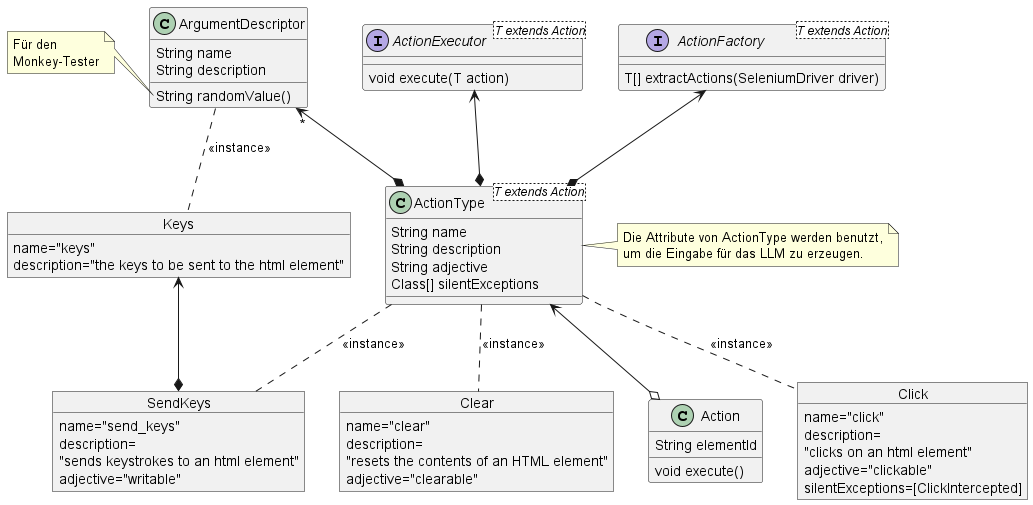
\includegraphics[width=0.9\textwidth]{plantuml/ActionType.png}
    \caption{Aufbau der Klasse \textit{ActionType}, mit der verschiedene Arten von Benutzerinteraktionen im Testscript repräsentiert werden.}
    \label{fig:actiontype}
\end{figure}

Das Testskript ist in Python geschrieben und verwendet die Bibliothek \textit{selenium} um den Browser zu steuern.
Es basiert auf dem Testskript von \Citeauthor{GPT3Testing} \cite{GPT3Testing}.
Die Implementierung der Monkey-Testers und das Kommandozeileninterface sind dabei größtenteils übernommen, die Extraktion der Interagierbaren Elemente und die Generierung für die Eingabe des LLM sind neu implementiert.
Im Gegensatz zum originalen Testskript werden außerdem verschiedene Arten von Benutzerinteraktionen unterstützt: Klicks und das Ausfüllen und Löschen von Formularfeldern.
Ursprünglich war auch das Hovern über Elemente möglich, das wurde aber aufgrund von Schwierigkeiten bei der Extraktion von Benutzerinteraktionen und der geringen Relevanz für die Evaluation des Ansatzes wieder entfernt.

Der Aufbau des Testscripts macht es einfach neue Arten von Benutzerinteraktionen hinzuzufügen.
Dafür gibt es die Klasse \textit{ActionType} (Abbildung \ref{fig:actiontype}), die die verschiedenen Arten von Benutzerinteraktionen repräsentiert und eine Referenz auf eine Methode hat, die die Interaktion ausführt.
Das Testscript hat eine statisch initialisierte Liste von \textit{ActionType} Instanzen, mit denen es eine Liste von möglichen Benutzerinteraktionen generiert.
Die Liste von \textit{ActionType} Instanzen kann erweitert werden, um neue Arten von Benutzerinteraktionen zu unterstützen.

Für den Monkey-Tester wird dann eine zufällige Benutzerinteraktion aus dieser Liste ausgewählt und ausgeführt.
Um eine Benutzerinteraktion mit dem LLM auszuwählen ist mehr Arbeit notwendig.
Die Eingabe des LLMs wird von dem Testscript dynamisch so erzeugt, dass die verschiedenen Arten von Benutzerinteraktionen erklärt werden und die dazugehörigen HTML-Elemente aufgelistet werden.
Dazu benutzt das Testscript die \textit{description} und \textit{adjective} (zu Deutsch: Beschreibung und Adjektiv) Attribute der \textit{ActionType} Instanzen.
Die \textit{description} ist eine Beschreibung der Benutzerinteraktion, die dem LLM erklärt, was diese Art von Benutzerinteraktion ist.

Normalerweise ist die Ausgabe der LLMs in natürlicher Sprache, aber in dieser Arbeit ist es notwendig, dass die Ausgabe des LLMs in einer speziellen Form ist, damit das Testscript die Ausgabe des LLMs interpretieren kann.
Dafür wird die \textit{Function-Calling} Schnittstelle von OpenAI verwendet, die es erlaubt, die Ausgabe des LLMs in einer speziellen Form zu erzeugen.
Function-Calling ist dafür gedacht, das LLM Funktion aufrufen zu lassen, die Argumente in Form von JSON-Objekten erwarten.
Die Form dieser JSON-Objekte lässt sich je nach Anwendungsfall mit Hilfe eines in einem \textit{JSON Schema}\footnote{\url{https://json-schema.org/}}-Dialekt definierten Schemas festlegen.
Die Modelle von OpenAI, die die Function-Calling Schnittstelle unterstützen sind so trainiert, dass sie die Argumente der Funktionen meistens in der richtigen Form ausgeben.
Dank dieser Schnittstelle ist es möglich, die von den \textit{ActionType} Instanzen generierten Benutzerinteraktionen zu verwenden, um dynamisch ein Schema zu definieren und die Ausgabe des LLMs in die richtige Form zu bringen.



\section{Extraktion von Interaktionsmöglichkeiten}

Für das Testen mittels LLM ist es notwendig, die möglichen Benutzerinteraktionen aus der HTML-Repräsentation der Anwendung zu extrahieren.
Ein Monkey-Tester könnte die Interaktionselemente zwar auch durch rein zufällige Maus und Tastaturaktionen finden, dann wären die Testergebnisse nicht mehr vergleichbar mit denen des LLMs.

Leider genügt es nicht, Interaktionselemente durch ihre HTML-Tags und -Attribute zu identifizieren, denn in der Praxis ist es schwierig, die Interaktionselemente zu identifizieren, die nicht verdeckt sind.
Außerdem ist es mittels JavaScript möglich und gängig, auch HTML-Elemente interagierbar zu machen, die nicht dazu gedacht sind.
Beispielsweise sind einige Knöpfe in der Testanwendung keine HTML-Buttons, sondern div-Elemente, die durch JavaScript-Event-Listener interagierbar sind.
Rein auf Basis des HTML-Dokuments ist es nicht möglich, zu erkennen, dass diese Elemente interagierbar sind.

Ich habe keine Möglichkeit gefunden, automatisch festzustellen, welche Elemente einer Webseite interagierbar sind.
Deshalb habe ich die Verantwortlichkeit für die Identifikation dieser Elemente auf den Entwickler der zu testenden Anwendung gelegt.
Für das Testframework, das ich entwickelt habe, ist es notwendig, dass benutzbare HTML-Elemente durch ein spezielles Attribut gekennzeichnet sind.

Um herauszufinden, welche dieser gekennzeichneten Elemente nicht verdeckt sind, habe ich ein Skript entwickelt, das mithilfe der Bibliothek \textit{Selenium}\footnote{\url{https://www.selenium.dev/}} direkt im Browser ausgeführt wird.
Es benutzt die DOM-API des Browsers, um abzufragen, welches Element an der Stelle eines gekennzeichneten Elements zuoberst liegt.
Das gekennzeichnete Element kann nicht verdeckt sein, wenn das oberste Element Nachfahre des gekennzeichneten Elements oder das Element selbst ist.
Für die Testanwendung reicht dieses Kriterium zwar aus, generell lassen sich aber Fälle konstruieren, in denen dieses Kriterium nicht ausreicht, oder nicht zutrifft:
Beispielsweise durch absolute Positionierung oder z-index kann es sein, dass ein Element, das nicht vollständig verdeckt ist, nicht als solches erkannt wird.
Oder wenn das gekennzeichnete Element vollständig von Kindelementen verdeckt ist, die selbst interagierbar sind, ist das gekennzeichnete Element nicht interagierbar.

\section{Prompt-Engineering}

Die Qualität der generierten Ausgabe eines LLM hängt stark von der Qualität der Eingabe ab, die dem LLM gegeben wird. \cite{chain-of-thought}
Prompt-Engineering ist die Kunst, eine Eingabe zu formulieren, die das gewünschte Verhalten des LLM hervorruft.
In dieser Arbeit habe ich mich auf die Entwicklung von Prompts konzentriert, die die Anwendung navigieren und testen.
Im Speziellen sind Eingaben, mit denen das LLM zu Anwendungszuständen navigiert, die von klassischen Monkey-Testern schwer zu erreichen sind, von Interesse.

Dazu vergleiche ich die Qualität der generierten Benutzerinteraktionen, wenn das LLM mit verschiedenen Eingaben aufgerufen wird.
Die Qualität der generierten Benutzerinteraktionen wird anhand der Branchenabdeckung gemessen, mehr dazu in Abschnitt \ref{sec:vaildation}.

\begin{enumerate}
    \item Basis-Eingabe: Die Basis-Eingabe ist ein einfacher Satz, der das LLM auffordert, eine Benutzerinteraktion zu generieren, die eine gegebene Webanwendung testen soll.
    \\
    Beispieleingabe:
    \\
    \textit{Du bist Tester für Webanwendungen und sollst eine gegebene Anwendung möglichst ausführlich testen.
    Hier ist die HTML-Repräsentation der Anwendung: ...
    Antworte mit einer der folgenden Benutzerinteraktionen: Klick auf \dq weiter\dq, Klick auf \dq zurück\dq.}
    \item Verkettung: Zusätzlich zur Basis-Eingabe wird jeweils die letzte Ausgabe des LLMs an die Eingabe angefügt.
    \\
    Beispieleingabe:
    \\
    \textit{System: Du bist Tester für Webanwendungen und sollst eine gegebene Anwendung möglichst ausführlich testen.
    Hier ist die HTML-Repräsentation der Anwendung: ...
    Antworte mit einer der folgenden Benutzerinteraktionen: Klick auf \dq weiter\dq, Klick auf \dq zurück\dq.
    \\
    LLM: Klick auf \dq weiter\dq
    \\
    System: Hier ist die neue HTML-Repräsentation der Anwendung: ... Bitte fahre mit dem Testen fort. Antworte mit einer der folgenden Benutzerinteraktionen: Klick auf \dq weiter\dq, Klick auf \dq zurück\dq.
    }
    \item Beschreibung: Zusätzlich zur Verkettung wird das LLM aufgefordert, eine Beschreibung des Anwendungszustands zu generieren. Diese wird dann mit in den folgenden Eingaben verkettet.
    \\
    Beispieleingabe:
    \\
    \textit{System: Du bist Tester für Webanwendungen und sollst eine gegebene Anwendung möglichst ausführlich testen.
    Hier ist die HTML-Repräsentation der Anwendung: ... 
    Gib eine kurze Beschreibung des Anwendungszustands an, dann antworte mit einer der folgenden Benutzerinteraktionen: Klick auf \dq weiter\dq, Klick auf \dq zurück\dq.
    \\
    LLM: Es wird ein Dialog mit dem Warnhinweis angezeigt, dass die Löschung des Benutzerkontos endgültig ist. Klick auf \dq weiter\dq
    \\
    System: Hier ist die neue HTML-Repräsentation ...
    }
    \item Begründung: Das Model wird dazu aufgefordert eine Begründung für die Entscheidung zur Nutzerinteraktion zu liefern.
    \\
    Beispieleingabe:
    \\
    \textit{System: Du bist Tester für Webanwendungen und sollst eine gegebene Anwendung möglichst ausführlich testen.
    Hier ist die HTML-Repräsentation der Anwendung: ... 
    Gib eine kurze Beschreibung des Anwendungszustands an, dann antworte mit einem Plan, was als nächstes getestet werden soll und einer der folgenden Benutzerinteraktionen, die dafür gewählt werden muss: Klick auf \dq weiter\dq, Klick auf \dq zurück\dq. 
    \\
    LLM: Es wird ein Dialog mit dem Warnhinweis angezeigt, dass die Löschung des Benutzerkontos endgültig ist.
    Teste das Löschen des Benutzerkontos.
    Klick auf \dq weiter\dq
    \\
    System: Hier ist die neue HTML-Repräsentation ...
    }
    \item
    Selbst formulierte Ziele: Das LLM wird dazu aufgefordert, Ziele zu formulieren, die es in der Anwendung erreichen soll.
    Diese Ziele sollen mehrere Benutzerinteraktionen umfassen.
    Jede Eingabe enthält das aktuelle Ziel, das sich das LLM gesetzt hat, sowie eine Aufstellung der Anzahl an Benutzerinteraktionen, die das LLM für jedes bisherige Ziel benutzt hat.
    \\
    Beispieleingabe:
    \\
    \textit{System: Du bist Tester für Webanwendungen und sollst eine gegebene Anwendung möglichst ausführlich testen.
    Hier ist die HTML-Repräsentation der Anwendung: ... 
    \\
    System: Gib eine kurze Beschreibung des Anwendungszustands an, dann stell zunächst abstraktes Ziel auf, das du über die nächsten Benutzerinteraktionen erreichen möchtest.
    Stelle dann einen Plan auf, wie das Ziel erreicht werden soll, gefolgt von einer Benutzerinteraktion, die dafür ausgeführt werden muss: Klick auf \dq weiter\dq, Klick auf \dq zurück\dq.
    \\
    System: Dein aktuelles Ziel ist: Teste die Funkionen des Benutzerkontos.
    \\
    System: Bisher hast du folgende Ziele verfolgt und Benutzerinteraktion ausgelöst: 9 Interaktionen für \glqq{}Teste die Funktionen des Benutzerkontos\grqq{}
    \\
    LLM: Es wird ein Dialog mit dem Warnhinweis angezeigt, dass die Löschung des Benutzerkontos endgültig ist.
    Neues Ziel: Teste das Erstellen neuer Kommentare.
    Plan: Bleibe eingeloggt und navigiere zu einem Artikel, der noch keine Kommentare hat. Schreibe einen Kommentar und überprüfe, ob er angezeigt wird.
    Klick auf \dq zurück\dq
    \\
    System: Hier ist die neue HTML-Repräsentation ...
    }
    \item Einsatz von \textit{Chain-of-Thought} bei Eingaben  \cite{chain-of-thought}:
    Diese spezifische Anforderung an das Format der Ein- und Ausgabe eines Sprachlernmodells verlangt, dass die generierten Inhalte einen tiefgehenden, erläuternden Gedankengang darstellen.
    Im Gegensatz zu den Ansätzen Nummer 4 und 5, bei dem eine direkte Antwort ohne eingebettete Beispiele generiert wird, verlangt dieser Ansatz auch, dass im Eingabetext explizite Beispiele eingeführt werden.
    Diese Beispiele dienen dazu, den Erklärungsprozess zu unterstützen und zu veranschaulichen, wie das Sprachmodell zu seiner Schlussfolgerung gelangen soll.
\end{enumerate}

\section{Validierung}
\label{sec:vaildation}

Um die Qualität der generierten Benutzerinteraktionen zu messen, wird die Testabdeckung der Testanwendung herangezogen.
Wie in \ref{sec:Foundations:TestCoverageMetrics} beschrieben, gibt es verschiedene Arten von Testabdeckung, die sich für verschiedene Anwendungsfälle eignen.
In dieser Arbeit wird die Branchenabdeckung verwendet, da speziell die Exploration von Anwendungszuständen und die Güte der Entscheidungen des LLMs von Interesse sind.
Wieviel Code tatsächlich ausgeführt wird, ist mehr oder weniger uninteressant, da dies von der Implementierung der Anwendung abhängt und nicht von der Qualität der generierten Benutzerinteraktionen.

Als Referenz für die Branchenabdeckung des Testens mittels LLM wird die Branchenabdeckung des Testens mittels eines Monkey-Tester herangezogen.
Der Monkey-Tester ist ein etabliertes Werkzeug, das zufällige Benutzerinteraktionen generiert und ausführt.
Monkey-Tester funktionieren in der Praxis meistens selbst schon sehr gut, aber sie sind aber manchmal nicht in der Lage, bestimmte Anwendungszustände zu erreichen.
Hier ist die Hoffnung, dass das LLM in der Lage ist, diese Anwendungszustände zu erreichen und eine höhere Branchenabdeckung zu erzielt.

Zur besseren Vergleichbarkeit wird die Branchenabdeckung in Prozent nach jeder simulierten Benutzerinteraktion gemessen.
Der Monkey-Tester generiert in manchen Implementierungen nur zufällige Klicks und Tastatureingaben generiert, was in im Vergleich ein massiver Nachteil wäre.
Deshalb ist er so implementiert, dass er nur \glqq{}sinnvolle\grqq{} sinnvolle Interaktionsmöglichkeiten auszuwählen kann, genau wie das LLM.
(Er kann als zum Beispiel nicht auf Text klicken, wenn der Klick keinen Effekt hätte.)
Das bedeutet, dass der Monkey-Tester und das LLM durch den gleichen Zustandsgraphen navigieren und die gleichen Anwendungszustände erreichen können.
In der Implementierung der Texterzeugung für Formularfeldern des Monkey-Testers wurde darauf geachtet, dass neben Zahlen und Buchstaben nur die Zeichen erzeugt werden, die notwendig sind um die Validierung des Bestellformulars zu bestehen.
Was streng genommen nicht dem Verhalten eines klassischen Monkey-Testers entspricht, aber zu höheren Testabdeckungen bei der Testanwendung führen sollte.

Wenn der LLM-Tester eine höhere Branchenabdeckung erreicht als dieser für die Testanwendung optimierte Monkey-Tester, dann ist das ein Hinweis darauf, dass das der LLM-Tester generell bessere Ergebnisse erzielen kann, als ein nicht optimierter Monkey-Tester.
Es wird nur mit den Modellen von OpenAI gearbeitet, die die Function-Calling Schnittstelle unterstützen.
An Stelle von GPT-4, welches teurer ist und sehr ähnliche Ergebnisse liefern sollte wie GPT-4-turbo, wird nur GPT-4-turbo verwendet.

%% ---------------------
%% | / Example content |
%% ---------------------